\documentclass[tikz,border=10pt]{standalone}
\usepackage{amsmath}
\begin{document}
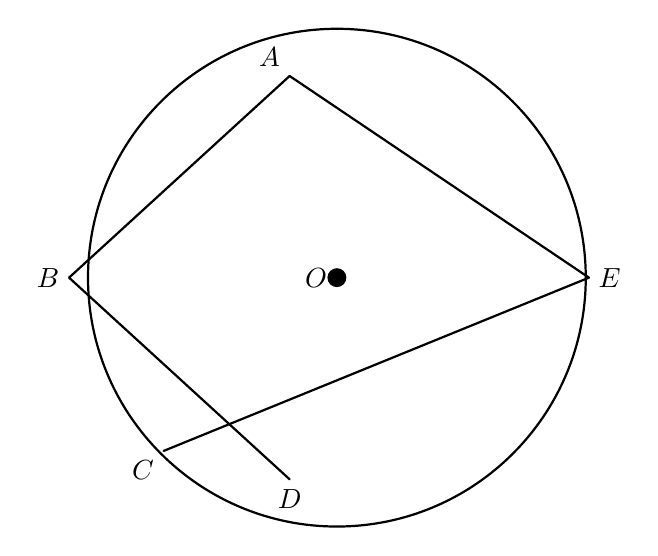
\begin{tikzpicture}[scale=0.02, line cap=round, line join=round]
  % Circle center and radius
  \coordinate (O) at (0,0);
  \coordinate (A) at (-30,128);
  \coordinate (B) at (-170,0);
  \coordinate (E) at (160,0);
  \coordinate (D) at (-30,-128);
  \coordinate (C) at (-110,-110);

  \draw[thick] (O) circle (158);

  \draw[thick] (B) -- (A);
  \draw[thick] (A) -- (E);
  \draw[thick] (B) -- (D);
  \draw[thick] (C) -- (E);

  \fill (O) circle (6);

  \node[above left] at (A) {$A$};
  \node[left] at (B) {$B$};
  \node[right] at (E) {$E$};
  \node[below] at (D) {$D$};
  \node[below left] at (C) {$C$};
  \node[left] at (O) {$O$};
\end{tikzpicture}
\end{document}
